\chapter{Optical modeling}
\label{chapter:optical_modeling}
A well-defined optical model can enhance the linearity of the sensor \cite{my_love_pressure_photosensor}. Therefore, this chapter will concentrate on the mathematical model of the optocoupler and the physical processes that determine the characteristics of an optical pressure sensor.

The primary components of the optocoupler include two phototransistors (PTs), a light-emitting diode (LED), and a photobarrier (PB). 
In optical pressure sensing, two PTs are utilized: one as a measuring device and the other as a reference. 
A barrier is positioned between the measuring PT and the LED. 
When pressure is applied to the barrier, it shifts and obstructs a portion of the light from the LED, thereby altering the induced current on the measuring PT.

The purpose of the chapter is to find the function $F = f(i_{\textit{mes pt}})$, which describes the relation between current on the measuring phototransistor $i_{\textit{mes pt}}$ and load $F$, applied to the barrier.
% Lets define the physical processes which are caused by change of the load on the PB. 

For the project I use a PT module (EE-SX1321, OMRON). 
The emitter and detector of the sensor consists of a set of cells as shown in Fig. \ref{fig:microscopic_image}.

\begin{figure}[H]
  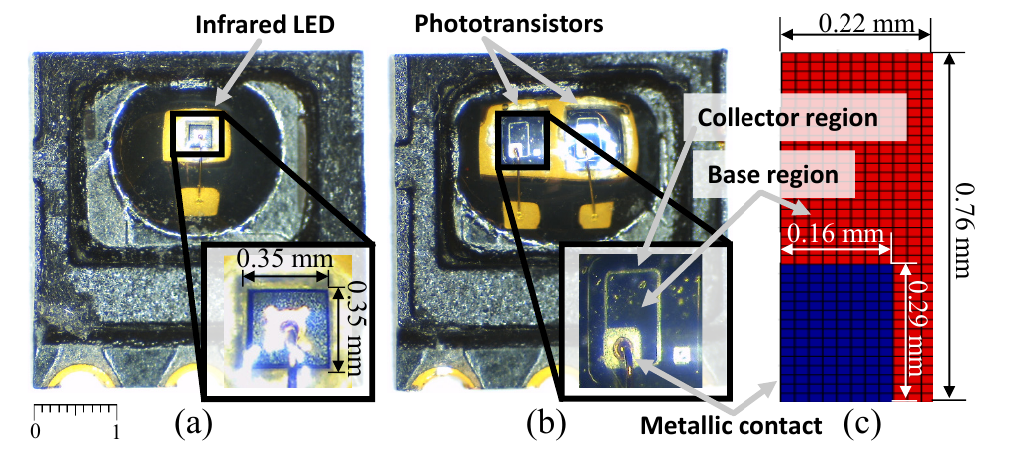
\includegraphics[width=\textwidth]{figs/Microscopic_image.png}
    \centering
    \caption{ Microscopic image showing (a) the LED and (b) the PTs embedded within the optocoupler (EE-SX1321, OMRON). 
    (c) Base area of the PT estimated by \cite[Fig. 4]{my_love_pressure_photosensor}.
    Adapted from \cite[Fig. 4]{my_love_pressure_photosensor}.}
    \label{fig:microscopic_image}
\end{figure}

% Optical model of my measurement cell wil be based on the one described in \cite{my_love_pressure_photosensor}.
In the upcoming chapter, the PB will be simplified to a spring element with an aperture. 
This simplification enables the use of Hooke's law $F = k\Delta d$, where F represents the load applied 
to the PB, $\Delta d$ denotes the shift of the barrier's aperture, and k represents the 
characteristic of the spring. 
By using this law, the function $F = f(i_{\textit{mes pt}})$ can be updated to $F = k \Delta d = k f_d(i_{\textit{mes pt}})$..
The value of k will be determined through finite element analysis (FEA) in the subsequent chapter. 

\begin{figure}[H]
  \centering
  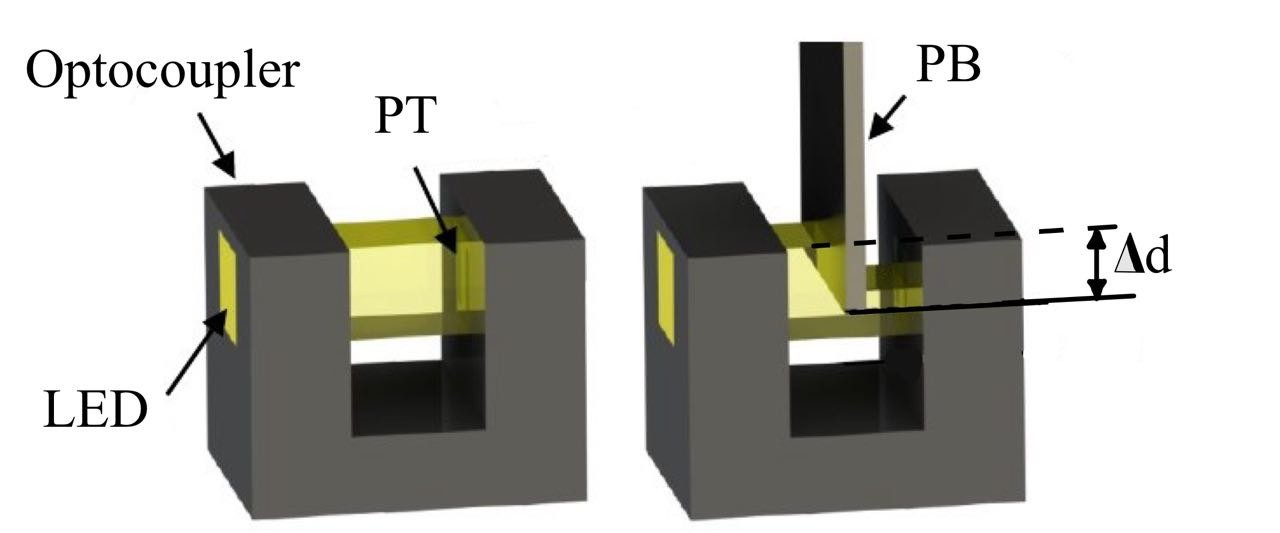
\includegraphics[width=0.7\textwidth]{illustration_of_PB_shift.jpg}
  \caption{Model of PT-based load sensing mechanism. Adapted from \cite[Fig. 1]{my_love_pressure_photosensor}.}
  \label{fig:load_pt_based_mechanism}
  \end{figure}

Limitations of the mathematical model:
\begin{itemize}
    \item LED is Lambert's source of light.
    \item PT acceptable wavelength is the same as of emitted light.
    \item Light is a stream of particles.
    \item PB will be simplified to the spring element with aperture. When a force is applied to the PB, the aperture will be shifted relative to the main optical axis of the light source.
\end{itemize}

\section{Optocoupler}
% \section{Geometric and optical model}
% ------------------------------------------
% IlluminanceFigure
Fig. \ref{fig:LED_PT_scetch} illustrates the geometric relationship between the LED and PT. 
As mentioned, the optocoupler's LED and PT are divided into small cells by hardware.
 Each cell of the LED will be treated as a Lambertian source of light, and the intensity 
 of PT cells will be calculated individually. 
 The overall intensity of the entire PT is then determined by summing these individual intensities. 

\begin{figure}[H]
  \centering
  \begin{subfigure}[b]{0.3\textwidth}
    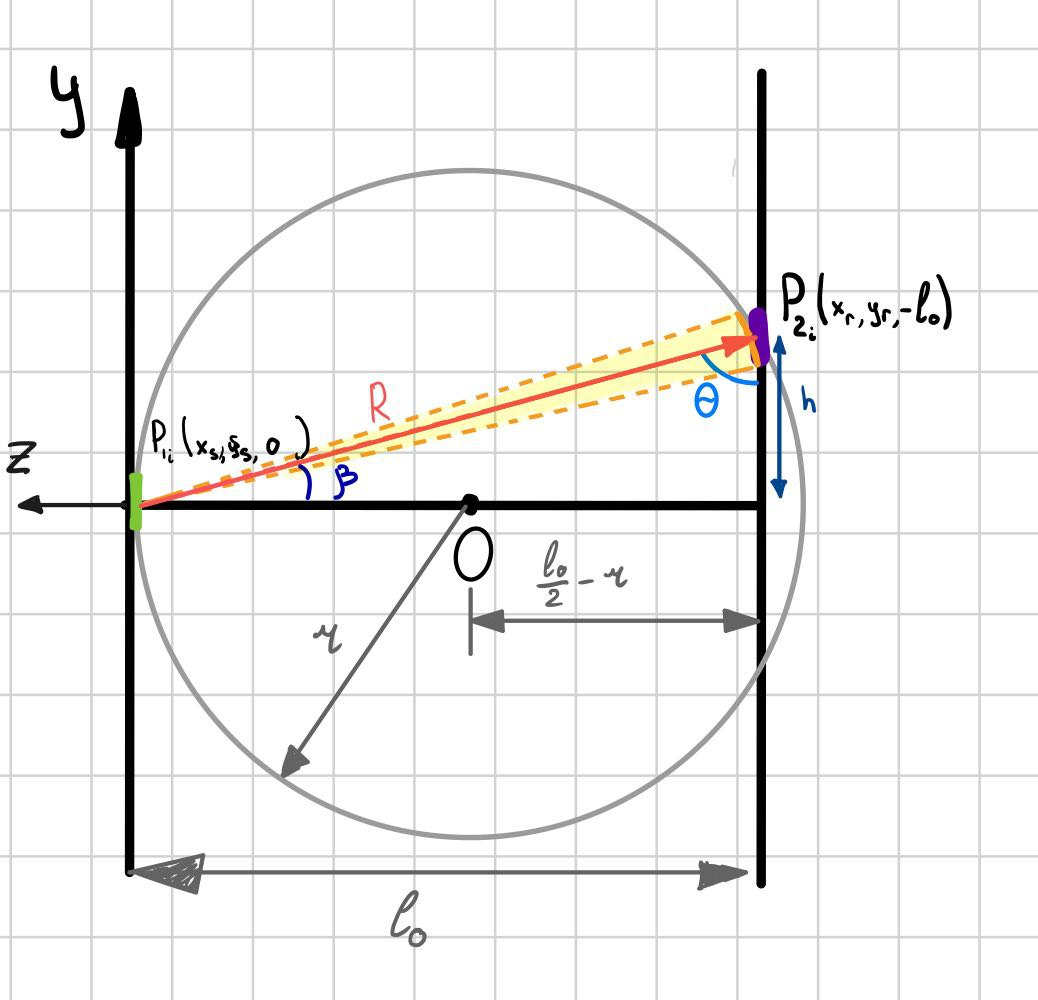
\includegraphics[width=\textwidth]{figs/simplified_model_notebook.jpg}
    \label{fig:sketch_ZY}
      \caption*{(a)}
    \end{subfigure}
    % \hfill
    \begin{subfigure}[b]{0.32\textwidth}
      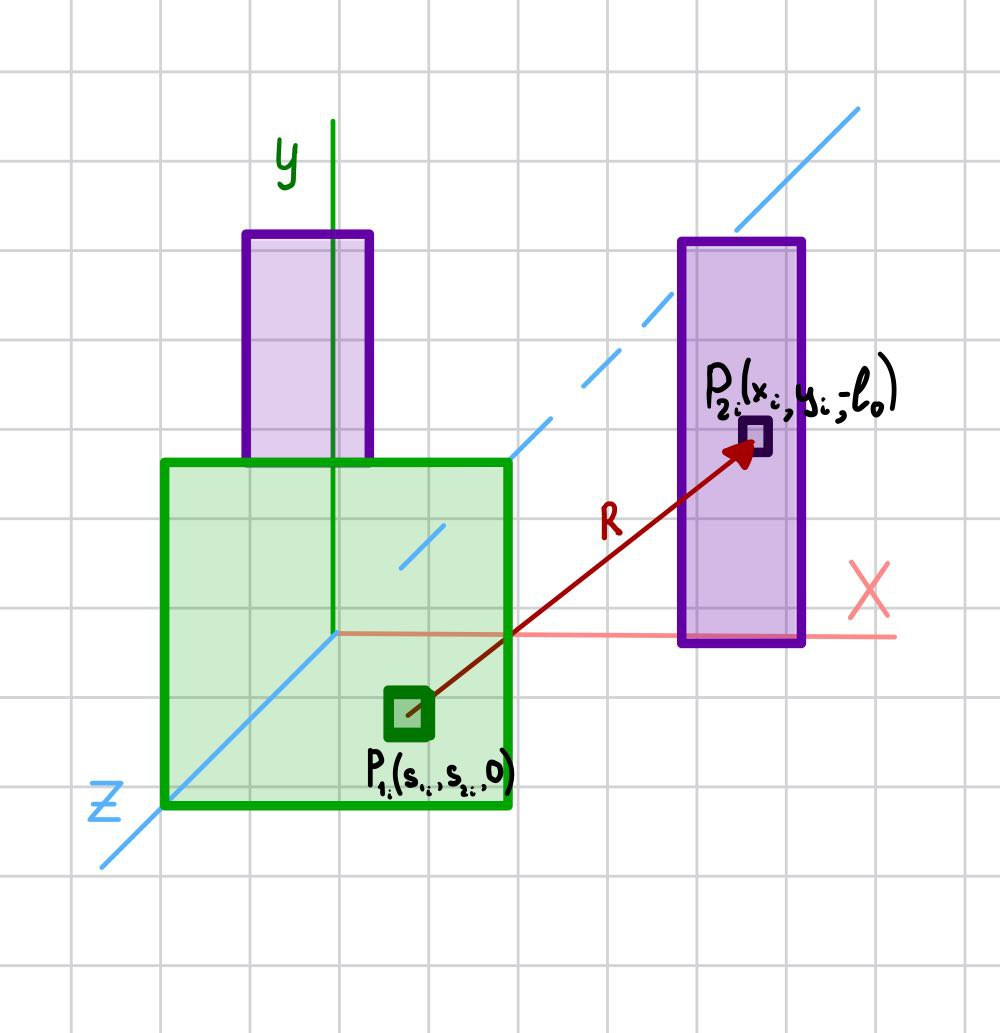
\includegraphics[width=\textwidth]{figs/oblique_draft.jpg}
      \label{fig:sketch_oblique}
      \caption*{(b)}
    \end{subfigure}
  \caption{Geometrical relationships between LED (green) and PT(purple): (a) YZ plane sketch, (b) oblique sketch.}
  \label{fig:LED_PT_scetch}
\end{figure}

To start with function $f_d(i_{\textit{mes pt}})$, it is important to note that $i_{\textit{mes pt}} 
\sim \Phi(\vec{r})$, where $\Phi(\vec{r})$ represents the amount of radiant power (radiation flux) passing through the area of interest, with its norm aligned with $\vec{r}$.

To incorporate the distance between the light emitter and receiver into the model, I will utilize luminous intensity, which indicates the level of brightness and determines the flux passing through a solid angle 
$\Omega$, proportional to the squared distance from the observer to the light source.

\[I(\vec{r}) = \frac{d\Phi}{d\Omega} \]
\[\Omega = \frac{A^\perp}{r^2}\]
The radiant intensity of a unit area of the LED exhibits Lambertian reflectance. 
Therefore, a unit surface of the application will receive an amount of radiation proportional to the cosine law:
\[I(\vec{r})_\perp = I_{0} cos (\beta)\]

The radiation pattern on a unit area perpendicular to the r vector will be as follows \cite{my_love_pressure_photosensor}:
\[I(\vec{r})_\perp = I_0 \frac{\cos{\beta}}{4 \pi r^2}\]

In our case, the PT surface is a sheet, which is why we need to project the calculated illuminance onto the PT plane: 
$$I(\vec{r}) = I_0 \frac{\cos^2{\beta}}{4 \pi r^2}$$

\[
h = (x_s- x_r)^2 + (y_s - y_r)^2\\
R^2 = h^2 + l_0^2\\
r^2  = h^2 + (\frac{l_0}{2})^2\\
\beta = \arcsin(\frac{h}{R})\\
\]

where $R$ - radius vector from $i$-th light source to the $j$-th receiver cell,
$\beta$ - angle between norm vector of emitter area and the vector R,
$s_1$ and $s_2$ - coordinates of the LED,
$x$ and $y$ - coordinates of the PT.

From the geometrical relationship, the total PT radiation flux is the integral of the LED ($A_{LED}$) and PT ($A_{PT}$) areas:

\begin{equation}
  \Phi = \int_{A_{LED}} \int_{A_{PT}} I(\vec{r})d A_{LED} d A_{PT}
  \label{eq:flux_calc}
\end{equation}
\begin{figure}[H]
    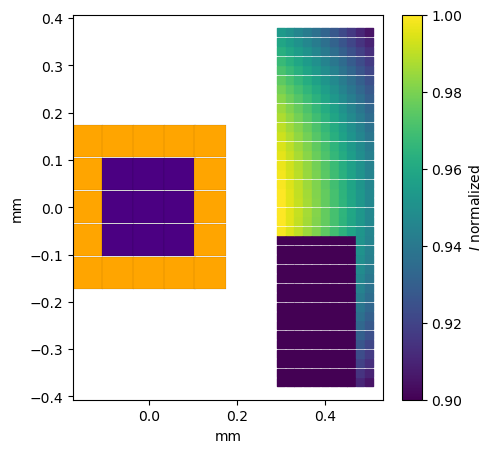
\includegraphics[width=0.5\textwidth]{output_with_one_pt.png}
      \centering
      \caption{Results of optical model simulation without PB (LED on the left, PT on the right). The purple color defines zones of optocoupler used for electrical connection (EE-SX1321, OMRON).}
      \label{fig:led_sim_res_one_pt}
\end{figure}

On the Fig. \ref{fig:led_sim_res_one_pt} results of the model simulation with one PT and a LED are presented.

% At the next step lets add to the model the PB.
\section{Photobarrier}
The Photo Barrier (PB) will be simplified to a cuboid shape, which will partially cover the phototransistor from the LED light. The relationship between the optocoupler and the PB is shown in Figure \ref{fig:load_pt_based_mechanism}. 
The stimulus for the pressure sensor depends on the shift of the photobarrier 
as its tip moves alongside the measuring PT. 
The PT module used (EE-SX1321, OMRON) has small dimensions, 
so the barrier shift is limited by the height of the PT, which is 0.76 mm as shown in Fig. \ref{fig:microscopic_image}. 
When the bottom edge of the PB reaches the borders of the PT, 
the intensity measurements will remain constant.

% To calculate the intensity of light on the PT cells with respect to PB, lets define geometric relationship between the amount of light passed to the receiver from a LED cell when a barrier is shifted.
% The model defines extremum $\boldsymbol{y_{\textit{PT}ext}}$ coordinate as $\boldsymbol{y}$ coordinate of barrier shadow on the PT. 
% So, the PB cells above the $\boldsymbol{y_{\textit{PT}ext}}$ do not receive light from the LED cell Fig. \ref{fig:extremum_ys_cell}.

% The model use not the $\boldsymbol{y_{\textit{PT}ext}}$, but the  $\boldsymbol{y_{\textit{LED}ext}}$ which is the coordinate of the LED the emmited light of which reaches the PT cell.
To calculate the intensity of light on the PT cells in relation to the PB, 
we define the geometric relationship between the amount of light transmitted 
to the receiver from an LED cell when a barrier is shifted. 
The model defines the extremum $\boldsymbol{y_{\textit{PT}ext}}$ coordinate as 
the $\boldsymbol{y}$ coordinate of the barrier shadow on the PT. 
Therefore, the PB cells above the $\boldsymbol{y_{\textit{PT}ext}}$ do not receive light
 from the LED cell.


The model uses not the $\boldsymbol{y_{\textit{PT}ext}}$, but the $\boldsymbol{y_{\textit{LED}ext}}$, 
which is the coordinate of the LED that emits light reaching the PT cell, as shown in Figure \ref{fig:extremum_ys_cell}..
\begin{figure}[H]
  \centering
  \begin{subfigure}[b]{0.3\textwidth}
    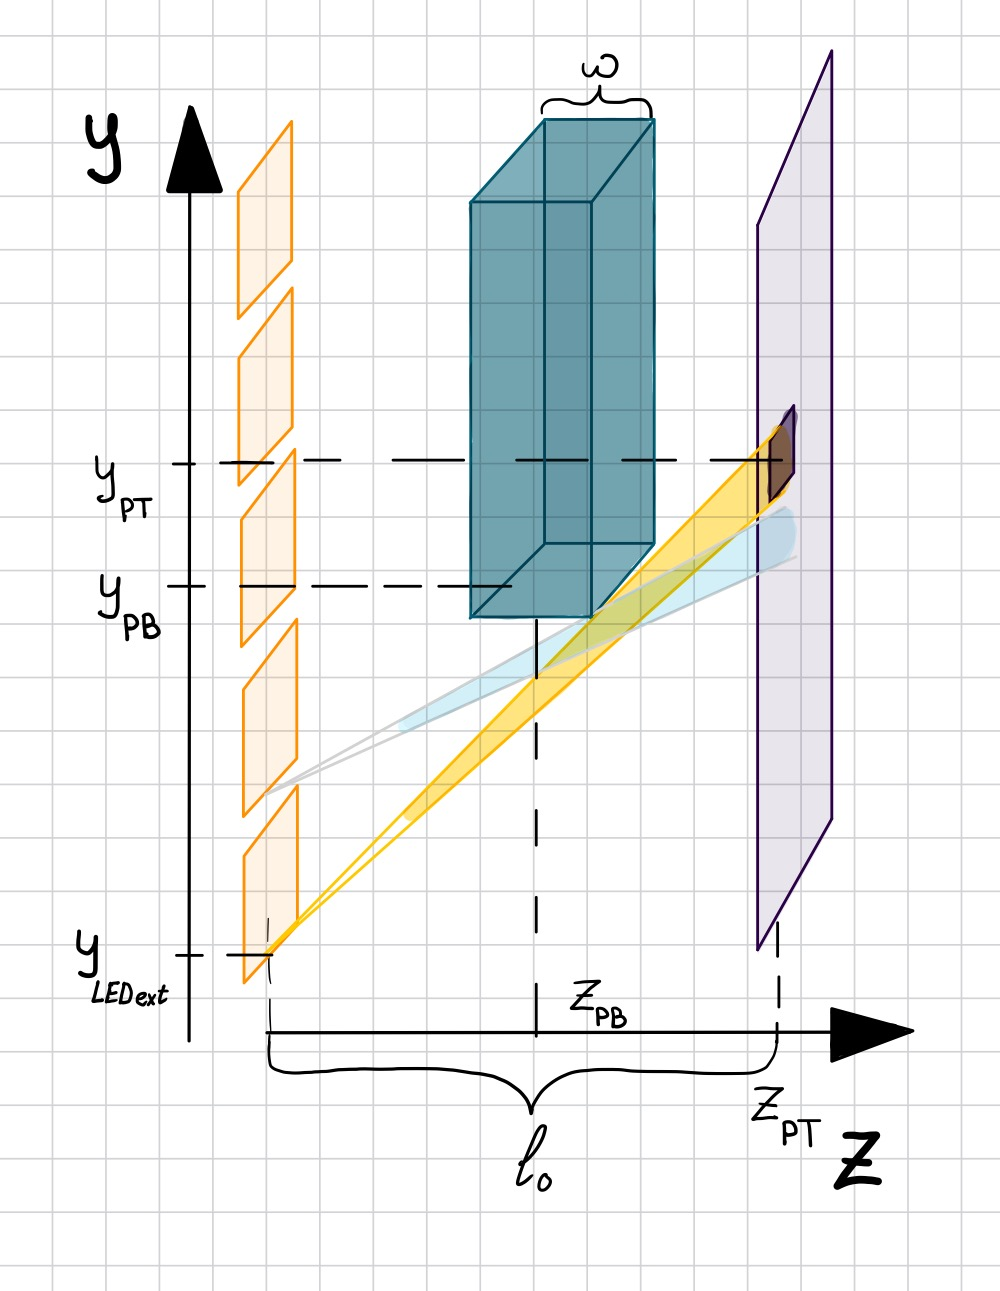
\includegraphics[width=\textwidth]{OM/barrier_geom_bott.jpg}
    \centering
    \label{fig:extremum_ys_cell_bottom}
    \caption*{(a)}
  \end{subfigure}
    % \hfill
  \begin{subfigure}[b]{0.35\textwidth}
    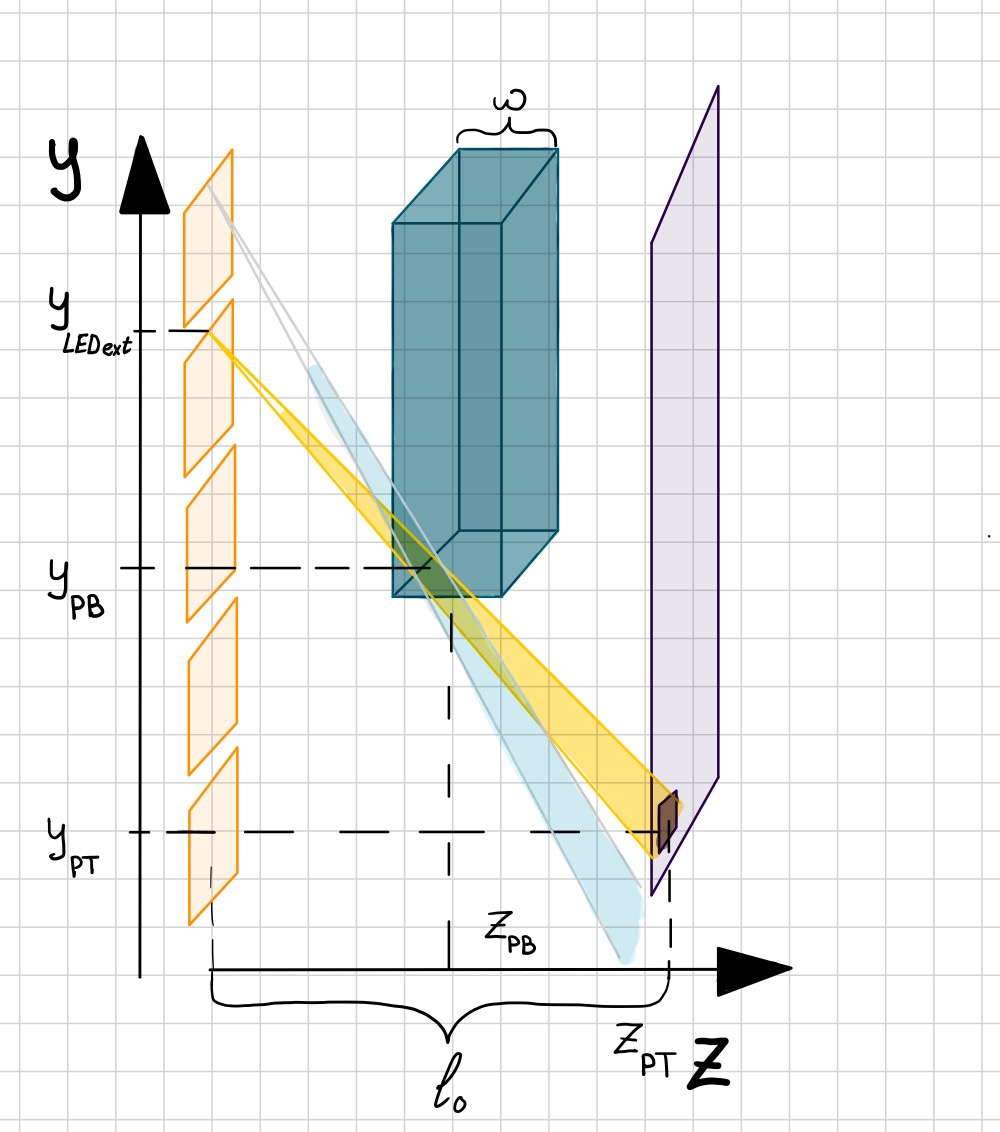
\includegraphics[width=\textwidth]{OM/barrier_geom_upp.jpg}
    \label{fig:extremum_ys_cell_upp}
    \caption*{(b)}
  \end{subfigure}
  \caption{Geometrical relationship between $\boldsymbol{y_{\textit{LED}ext}}$, photobarrier and phototransistor cells: (a) $y_{PT} > y_{PB}$, (b)  $y_{PT} < y_{PB}$ }
  \label{fig:extremum_ys_cell}

\end{figure}

The extremum $\boldsymbol{y_{\textit{LED}ext}}$ is calculated for each PT cell is defined as the following:

$$
  \Delta y = y_{PB} - y_{PT}\\
$$
$$
  \begin{cases}
    \Delta z = z_{PB} + (\omega / 2), &  \text{if }y_{PT} > y_{PB}\\
    \Delta z = z_{PB} - (\omega / 2)  & \text{otherwise}
  \end{cases}\\
$$
$$
  \boldsymbol{y_{\textit{LED}ext}} = \frac{\Delta y  l_0}{\Delta z}
$$

where $y_{PB}$, $z_{PB}$ - y, z coordinated of PB cell, 
$y_{PT}$ - y coordinate of the PT cell,
$l_0$ - distance between PT and LED,
$\omega$ - barrier thickness.

From Fig. \ref{fig:extremum_ys_cell} one can see that the light from a LED cell with coordinated ($ x_{LED}, y_{LED}$) reaches the PT cell if $y_{LED} < \boldsymbol{y_{\textit{LED}ext}}$.
Therefore the total PT radiation flux Eq. \ref{eq:flux_calc} updates up to:

\begin{equation}
  \Phi = \int_{A_{LED}} \int_{A_{PT}} I(\vec{r})d A_{LED} d A_{PT} = \sum_{}^{A_{LED}} \sum_{}^{A_{PT}} \begin{cases}
    I(\vec{r}), & \text{if }y_{LED} < \boldsymbol{y_{\text{LED}ext}}\\
    0, & \text{otherwise}
  \end{cases}
  \label{eq:flux}
\end{equation}

\begin{figure}[H]
  \centering
  \begin{subfigure}[b]{0.3\textwidth}
    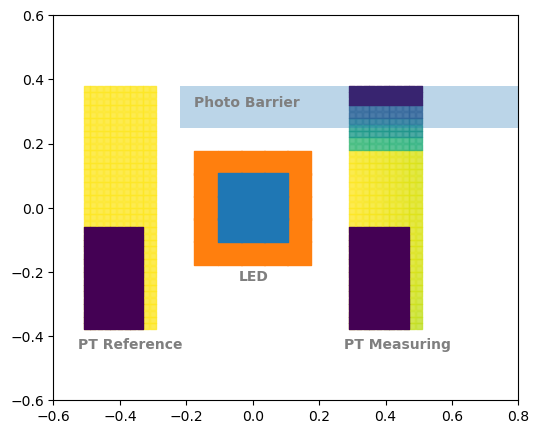
\includegraphics[width=\textwidth]{0_25_y_barrier.png}
    \centering
    \label{fig:0_25_y_barrier}
    \caption*{(a)}
  \end{subfigure}
    % \hfill
  \begin{subfigure}[b]{0.3\textwidth}
    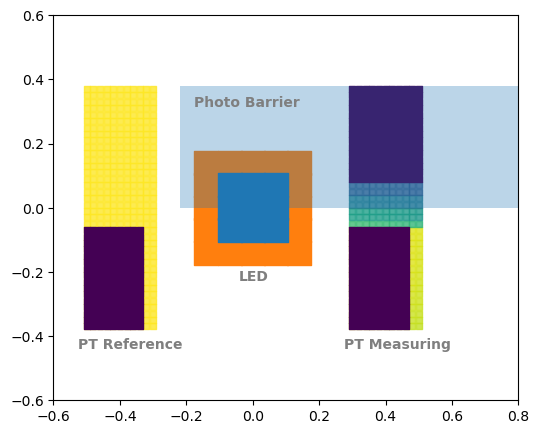
\includegraphics[width=\textwidth]{0_y_barrier.png}
    \label{fig:0_y_barrier}
    \caption*{(b)}
  \end{subfigure}
  \begin{subfigure}[b]{0.3\textwidth}
    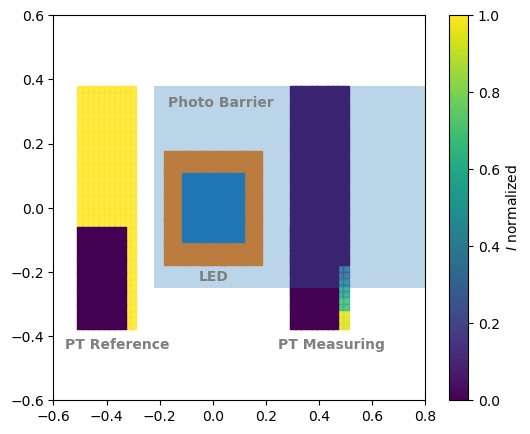
\includegraphics[width=\textwidth]{min_0_25_y_barrier.png}
    \label{fig:min_0_25_y_barrier}
    \caption*{(c)}
  \end{subfigure}
  \label{fig:LED_PT_simulation_vs_bar}
  \caption{Simulation with PB results for different barrier aperture shift: (a) 0.15 mm, (b) 0.4 mm, (c) 0.65 mm.}
\end{figure}


On the Fig. \ref{fig:LED_PT_simulation_vs_bar} the change of flux on the phototransistor is presented. The results are correlateed to the results, received by the researches in 
\cite{my_love_pressure_photosensor}.

% \begin{figure}[H]
%     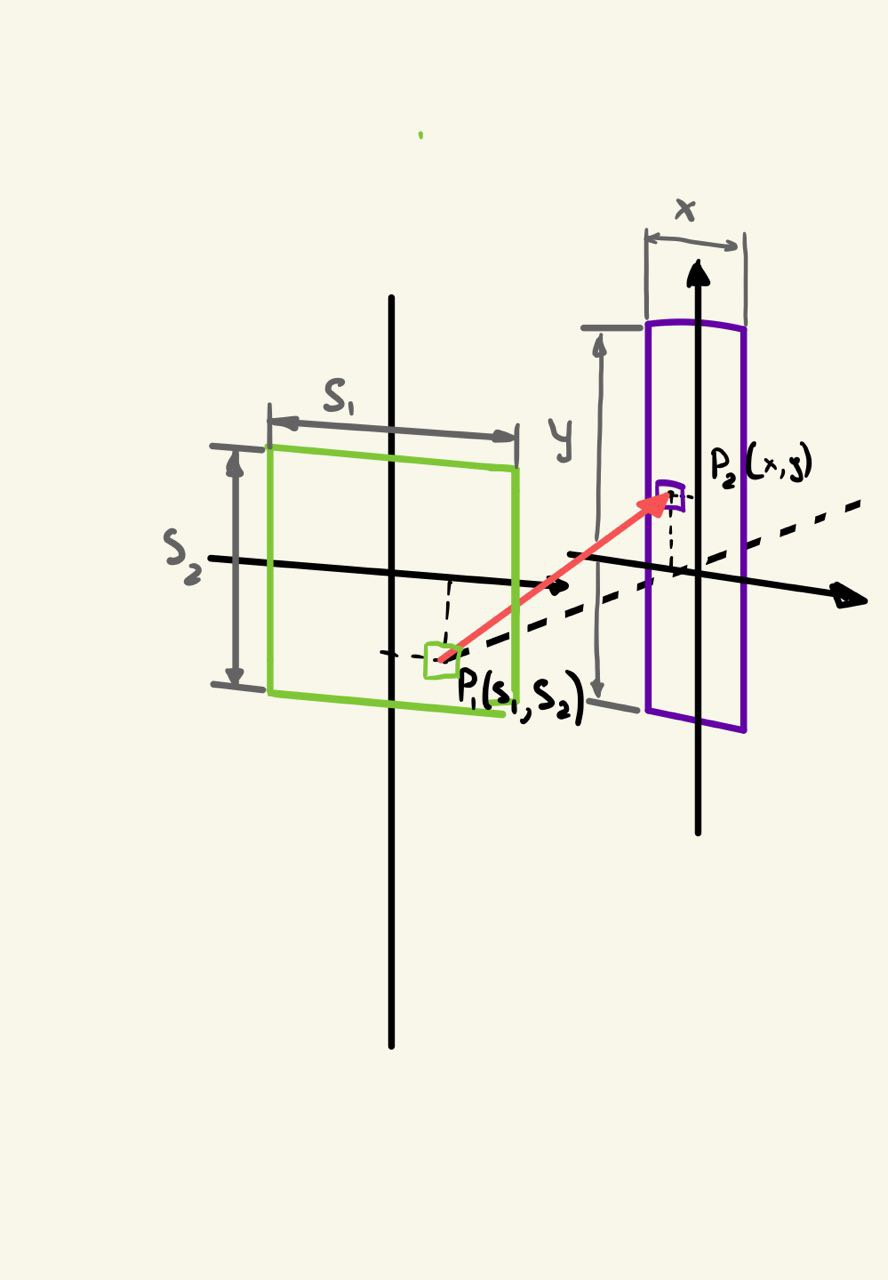
\includegraphics[width=0.5\textwidth]{figs/arrangement_of_LED_PT.jpg}
%         \centering
%         \caption{LED (green) and photoreceiver (purple) arrangement} 
%         \label{fig:arrangement_of_LED_PT}
%     \end{figure}
    
% \begin{figure}[H]
%     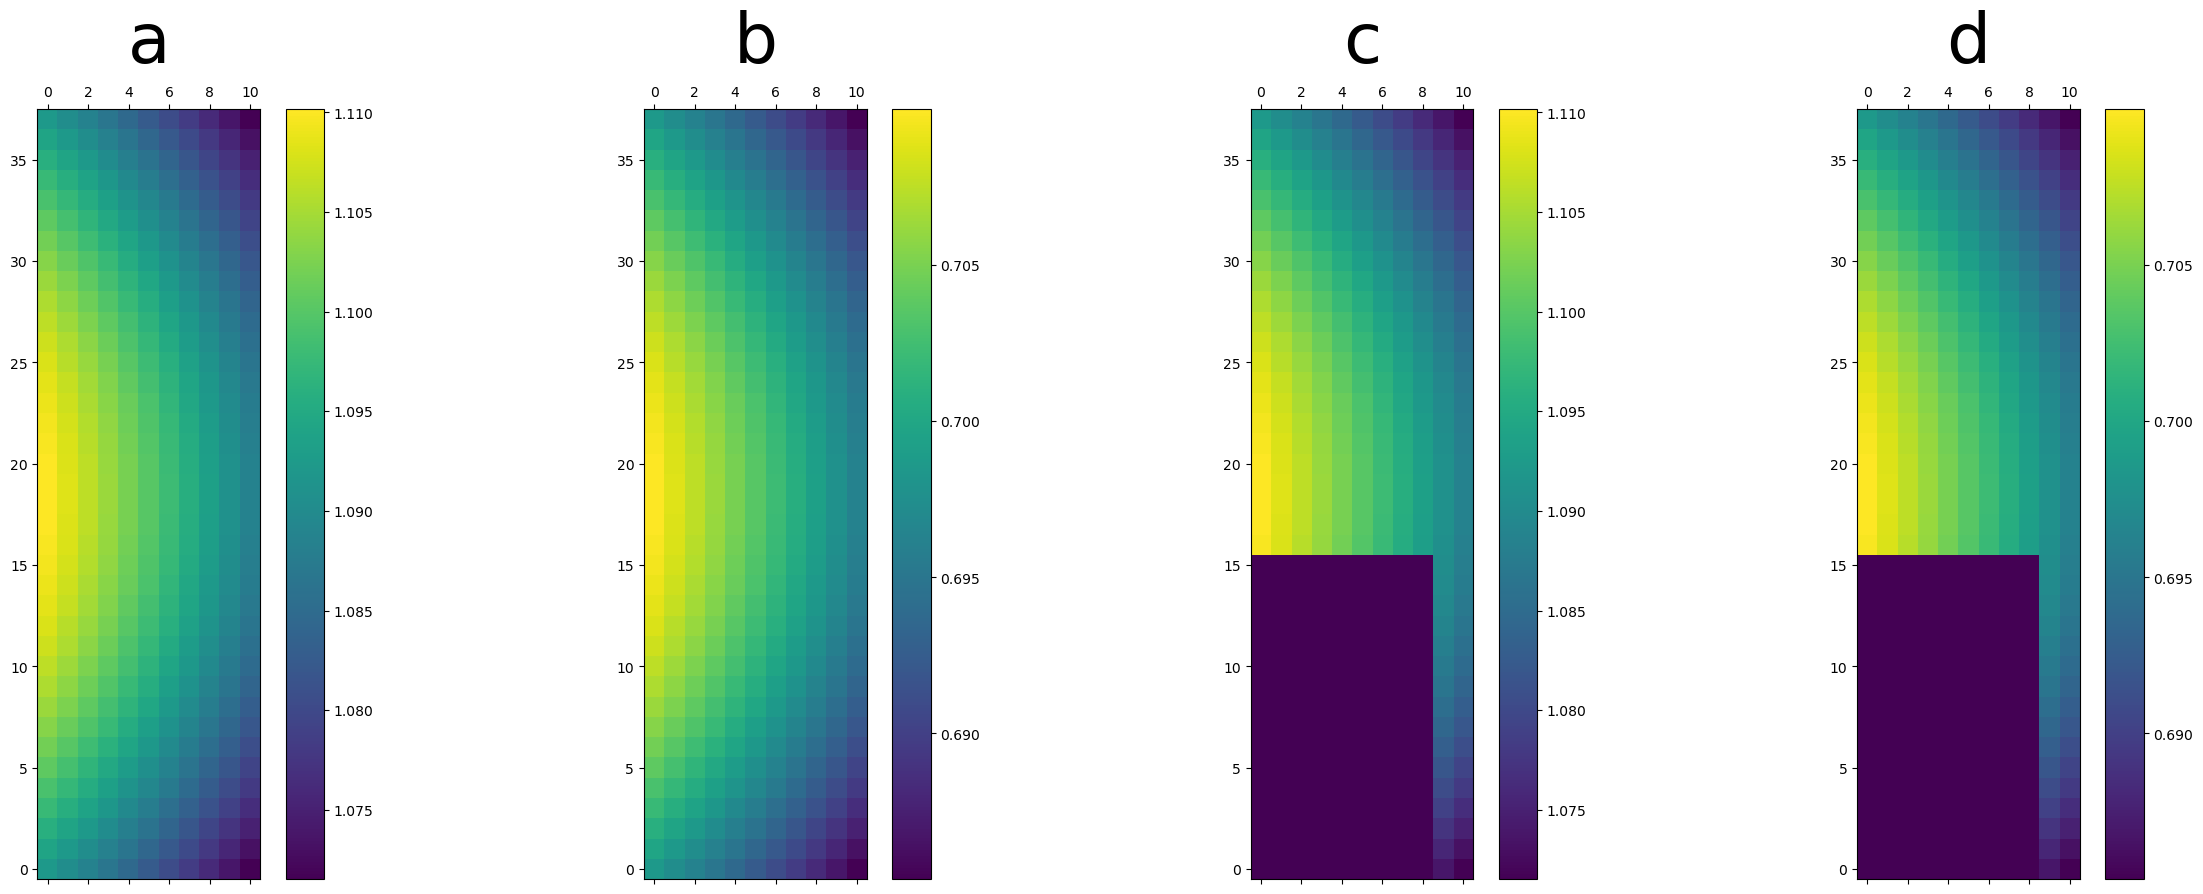
\includegraphics[width=1\textwidth]{figs/intensity_output.png}
%       \centering
%       \caption{Photoreceiver intensity from the formulas: a. The intensity of the }
%       \label{fig:intensity_output}
%     \end{figure}
    
% -------------------------------------------

% How to calculate the light intensity on the receiver area (flux)?

% The model should include area of the emitter and receiver since we measure the current change on the PT

% Illuminance estimates the flux received by some area. 
